\documentclass[../main/main.tex]{subfiles}

\newdate{date}{26}{10}{2020}

% \begin{figure}[h!]
% \centering
% \includegraphics[page=6,width=0.8\textwidth]{../lessons/pdf_file/11_lecture.pdf}
% \end{figure}

%\displaydate{date}. Compiled:  \today. Alice.

\begin{document}

\pagestyle{plain}

\section{Lecture 11}


\subsubsection*{Slide 1}

\begin{minipage}[]{0.5\linewidth}
\centering
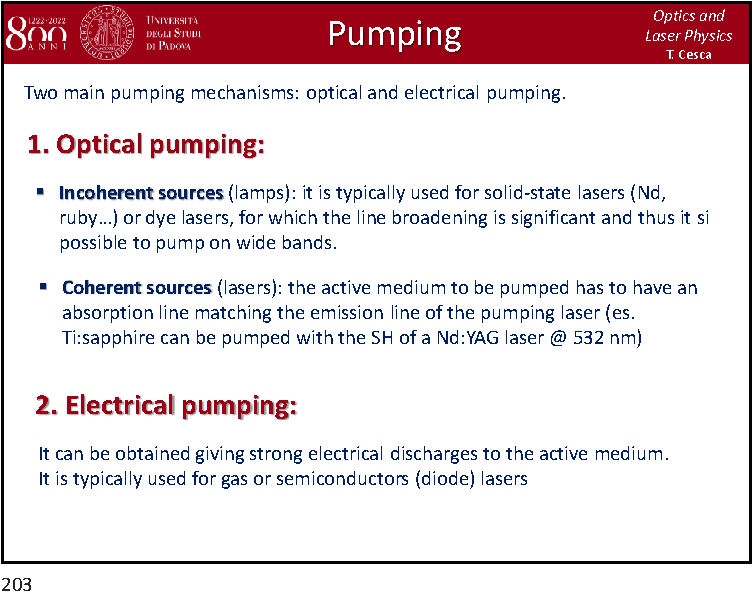
\includegraphics[page=1,width=1\textwidth]{../lessons/pdf_file/11_lecture.pdf}
\end{minipage}
\hspace{0.3cm}\vspace{0.3cm}
\begin{minipage}[c]{0.47\linewidth}

Out-of-equilibrium condition is provided by \textbf{pumping}.

We distinguish between:

\begin{itemize}
\item \textbf{optical pumping}.

\begin{itemize}
\item \textbf{incoherent sources}: when you have an active medium with a significant line broadening. In this way you can pump your medium on a wide band. These are the most common.

\item \textbf{coherent sources}: as lasers. Reach the condition in which the absorption line of the medium you want to pump has to match the emission line of the laser. This techniques is becoming popular because now we have a large variety of diode lasers (it is more easily to find the emission line which match) and they are becoming more powerful.

\end{itemize}

\item \textbf{electrical pumping}: used for gas and semiconductor lasers.

\end{itemize}

\end{minipage}

\subsubsection*{Slide 2}

\begin{minipage}[]{0.5\linewidth}
\centering
\includegraphics[page=2,width=1\textwidth]{../lessons/pdf_file/11_lecture.pdf}
\end{minipage}
\hspace{0.3cm}\vspace{0.3cm}
\begin{minipage}[c]{0.47\linewidth}

There are other possible pumping mechanism, but these are not too much used for common lasers because they require very expensive setups.

We will give some ides of optical pumping systems.

\end{minipage}

\subsubsection*{Slide 3}

\begin{minipage}[]{0.5\linewidth}
\centering
\includegraphics[page=3,width=1\textwidth]{../lessons/pdf_file/11_lecture.pdf}
\end{minipage}
\hspace{0.3cm}\vspace{0.3cm}
\begin{minipage}[c]{0.47\linewidth}

The Ruby laser used a \textbf{spiral lamp} in order to obtain the pumping. There are other possibilities. Now, it is more common to have an \textbf{elliptical cavity} configuration. The acitve medium is the \textbf{rod} and we use a \textbf{lamp} with a cylindrical shape. They are in the two focal points of the ellipses. For the other of the ellipse, the light of the lamp is reflected to the rod. To realize it, the cavity has to have reflective surfaces.

When we are talking about \textbf{cavity} we refer to the \textbf{pumping} one (not the resonant one in which we have the photon moving back and forward).

We can also realize a \textbf{close coupling} configuration, in which the lamp and rod are placed much closer. The surface of the cavity outside it an highly scattering surface (so it is no more reflective, in such a way it is without the risk of forming hotspots) to illuminate more uniformly.

\end{minipage}

\newpage

\subsubsection*{Slide 4}

\begin{minipage}[]{0.5\linewidth}
\centering
\includegraphics[page=4,width=1\textwidth]{../lessons/pdf_file/11_lecture.pdf}
\end{minipage}
\hspace{0.3cm}\vspace{0.3cm}
\begin{minipage}[c]{0.47\linewidth}

We have the \textbf{double-elliptical cavity} in which we use one rod and \textbf{two} lamps. There is the corresponding \textbf{close coupling} configuration.

\end{minipage}

\subsubsection*{Slide 5}

\begin{minipage}[]{0.5\linewidth}
\centering
\includegraphics[page=5,width=1\textwidth]{../lessons/pdf_file/11_lecture.pdf}
\end{minipage}
\hspace{0.3cm}\vspace{0.3cm}
\begin{minipage}[c]{0.47\linewidth}

These are schemes for lasers used in industry. The beam is propagating trhough active medium by total internal reflaction and the lamps provide the pumping so keep the active medium in the excited state.

\end{minipage}

\subsubsection*{Slide 6}

\begin{minipage}[]{0.5\linewidth}
\centering
\includegraphics[page=6,width=1\textwidth]{../lessons/pdf_file/11_lecture.pdf}
\end{minipage}
\hspace{0.3cm}\vspace{0.3cm}
\begin{minipage}[c]{0.47\linewidth}

Let us consider a four-level system.
The variation of the population due to pumping is reported.

It is possible to introduce the \textbf{pumping efficiency}: it is the product of different efficiencies. It is the ratio between the minimum power necessary to obtain laser transition (to populate upper level) \( p_m \) divided by the electric power that it is given to the system \( p_p \).

The \textbf{radiative efficiency} is the fraction of the emitted spectrum of the lamp which matches the absorption spectrum of your active medium.

The \textbf{transfer efficiency} is the fraction of the radiative emission of the lamp that matches the spectral range for pumping your active medium which is really transferred to the active medium. It depends on the configuration in which you place your pump and active medium.

\end{minipage}

The \textbf{absorption efficiency} is the fraction of the intensity that is coming from the lamp which is transferred to the active medium which is absorbed by the active medium.

The \textbf{power quantum efficiency}: how much of the absorbed energy is used to pump the upper laser level.

\( A l \)  is the volume of the active medium. \( \nu _{mp} \) is the minimum energy difference between the ground state and the upper laser level.

\newpage

\subsubsection*{Slide 7}

\begin{minipage}[]{0.5\linewidth}
\centering
\includegraphics[page=7,width=1\textwidth]{../lessons/pdf_file/11_lecture.pdf}
\end{minipage}
\hspace{0.3cm}\vspace{0.3cm}
\begin{minipage}[c]{0.47\linewidth}

If we are able to estimate the pumping efficiency, we can calculate the \textbf{pumping rate} necessary to get the population on the upper laser level.

\end{minipage}

\subsubsection*{Slide 8}

\begin{minipage}[]{0.5\linewidth}
\centering
\includegraphics[page=8,width=1\textwidth]{../lessons/pdf_file/11_lecture.pdf}
\end{minipage}
\hspace{0.3cm}\vspace{0.3cm}
\begin{minipage}[c]{0.47\linewidth}

A lot of work is required for the design of pumping system in order to obtain pumping efficiency as large as possible. Only a few percent of the pumping power is actually used to obtain laser action. This is a very \textbf{critical point}.

\end{minipage}

\subsubsection*{Slide 9}

\begin{minipage}[]{0.5\linewidth}
\centering
\includegraphics[page=9,width=1\textwidth]{../lessons/pdf_file/11_lecture.pdf}
\end{minipage}
\hspace{0.3cm}\vspace{0.3cm}
\begin{minipage}[c]{0.47\linewidth}

This is the section of a \textbf{rod} with refractive index \( n \) and radius \( R \). It is illuminated from a lamp. You cannot enter in the rod at angle larger than the critical angle.

At the critical angle, the ray is coming parallel to the surface. By considering the cylindrical geometry, we are using only the internal cylinder of the rod. In this way, a very limited portion of the road is used and the part outside the radius of \( R/n \) is not used.

\end{minipage}

\subsubsection*{Slide 10}

\begin{minipage}[]{0.5\linewidth}
\centering
\includegraphics[page=10,width=1\textwidth]{../lessons/pdf_file/11_lecture.pdf}
\end{minipage}
\hspace{0.3cm}\vspace{0.3cm}
\begin{minipage}[c]{0.47\linewidth}

To overcome this problem there are two possibilities:
\begin{itemize}
\item to reduce the reflectivity of the surface of the rod

\item create a \textbf{cladding} around with a thickness. If the total radius of the cylinder is \( n R \), the radius we use is exactly \( R \) and we are illuminating our rod completely.

\end{itemize}


\end{minipage}

\subsubsection*{Slide 11}

\begin{minipage}[]{0.5\linewidth}
\centering
\includegraphics[page=11,width=1\textwidth]{../lessons/pdf_file/11_lecture.pdf}
\end{minipage}
\hspace{0.3cm}\vspace{0.3cm}
\begin{minipage}[c]{0.47\linewidth}

Let us consider \textbf{laser pumping}:

\begin{itemize}
\item \textbf{longitudinal} pumping: the pumping laser is aligned with optical cavity of the laser to pump. The intensity of the laser beam \( I_p (r,z) \) depends on the propagation direction \( z \) and \( r \) the position on the perpendicular plane wrt propagation direction.

\item \textbf{transverse} pumping: the pumping laser is aligned perpendicularly to the optical cavity of the laser to pump.
It is not used very much, it does not guarantee a useful pumping.
To determine the pumping rate the integration along the volume of the active medium is required.

\end{itemize}

\end{minipage}

The \textbf{incidence pump power} \( P_{pi} \) is given by the product of \textbf{radiative efficiency}, \textbf{transfer efficiency} multiplied by the \textbf{electrical power of the pump laser}.

\subsubsection*{Slide 12}

\begin{minipage}[]{0.5\linewidth}
\centering
\includegraphics[page=12,width=1\textwidth]{../lessons/pdf_file/11_lecture.pdf}
\end{minipage}
\hspace{0.3cm}\vspace{0.3cm}
\begin{minipage}[c]{0.47\linewidth}

Also for \textbf{electrical pumping} we can distinguish:

\begin{itemize}
\item \textbf{longitudinal} pumping: the electrical discharge is produced longitudinally wrt the optical cavity of the laser. It provides uniform pumping but requires high voltages.

\item \textbf{transverse} pumping: the electrical discharge is produced perpendicularly wrt the axis of the optical cavity. Lower voltages are required, but it is more difficult to obtain an homogeneous pumping.

\end{itemize}

You have a distribution of locally pumping rate so you calculate the average \( \expval{R_p}  \).

\end{minipage}

\subsubsection*{Slide 13}

\begin{minipage}[]{0.5\linewidth}
\centering
\includegraphics[page=13,width=1\textwidth]{../lessons/pdf_file/11_lecture.pdf}
\end{minipage}
\hspace{0.3cm}\vspace{0.3cm}
\begin{minipage}[c]{0.47\linewidth}

From now, we will talk about the \textbf{optical cavity}, or \textbf{optical resonator}.

\textbf{Laser modes} are stationary configurations of electromagnetic field which obey Maxwell's equations within the cavity with boundary condition given by the presence of the mirror in the cavity.

We can distinguish longitudinal and transverse modes. Any time a laser oscillates, if \textbf{you do not do anything specific}, you will not select any modes, nor longitudinal nor transverse. So, when the laser is active the system is oscillating in a very large number of modes. The laser beam will be the \textbf{convolution} of all these configurations.

\end{minipage}

Let us consider the \textbf{Fabry-Perot cavity}. The wavelength of the modes supported by the cavity are only the one for which the length of the cavity is a multiple of \( \lambda /2 \). We have multiple frequency that can be sustainable bu this cavity, the others will be damped. The frequency different between two adjoint modes is given by \( \Delta \nu  = c / (2L) \).

\subsubsection*{Slide 14}

\begin{minipage}[]{0.5\linewidth}
\centering
\includegraphics[page=14,width=1\textwidth]{../lessons/pdf_file/11_lecture.pdf}
\end{minipage}
\hspace{0.3cm}\vspace{0.3cm}
\begin{minipage}[c]{0.47\linewidth}

For a more real cavity, in which we have two mirrors but with the active medium inside, we have to consider the \textbf{effective length} of the cavity (we are assuming to be in air \( n=1 \) where the active medium is not present).

Usually, the small in frequency is very small.

\end{minipage}

\subsubsection*{Slide 15}

\begin{minipage}[]{0.5\linewidth}
\centering
\includegraphics[page=15,width=1\textwidth]{../lessons/pdf_file/11_lecture.pdf}
\end{minipage}
\hspace{0.3cm}\vspace{0.3cm}
\begin{minipage}[c]{0.47\linewidth}

We can calculate the condition for more complicated cavities as \textbf{3-mirror} of \textbf{4-mirror}. The \textbf{effective perimeter} of the cavity has to be considered.

\end{minipage}

\subsubsection*{Slide 16}

\begin{minipage}[]{0.5\linewidth}
\centering
\includegraphics[page=16,width=1\textwidth]{../lessons/pdf_file/11_lecture.pdf}
\end{minipage}
\hspace{0.3cm}\vspace{0.3cm}
\begin{minipage}[c]{0.47\linewidth}

You have many difference cavity modes that can be amplified in the system, with a small frequency difference \( \Delta \nu  \).

However, all the cavity modes below the \textbf{gain bandwidth} (of active the medium) can be amplified by the active medium. By combining the optical resonator with the active medium, the modes that can be amplified are not infinite.

\end{minipage}

\subsubsection*{Slide 17}

\begin{minipage}[]{0.5\linewidth}
\centering
\includegraphics[page=17,width=1\textwidth]{../lessons/pdf_file/11_lecture.pdf}
\end{minipage}
\hspace{0.3cm}\vspace{0.3cm}
\begin{minipage}[c]{0.47\linewidth}

\textbf{Longitudinal modes} are frequency that can be amplified by the optical resonator and the active medium. Along the propagation direction the presence of the optical cavity define the frequency that are sustained by the cavity itself.

But, also \textbf{transverse modes} exist. They are the possible configuration in the plane perpendicular to the propagation direction. In the plane perpendicular to the axis of the optical cavity, there are only possible modes that can be obtained. In this case the demonstration is complicated and we look only the result.
After a certain number of oscillation back and forth within the cavity, the electromagnetic field will converge to a \textbf{stationary condition} has shapes like the ones in figure. The complexity increases for increasing the order of these modes (increasing the number of nodes within the profile). These are called \textbf{TEM} (transverse electromagnetic) modes.

\end{minipage}

These configurations are \textbf{independently} on the \textbf{shape} of the \textbf{electromagnetic field} you consider! They are reached almost immediatly. If you do nothing, the system will oscillate with all these nodes at the same time. The intensity distribution is the \textbf{overlap} between all these modes.

\subsubsection*{Slide 18}

\begin{minipage}[]{0.5\linewidth}
\centering
\includegraphics[page=18,width=1\textwidth]{../lessons/pdf_file/11_lecture.pdf}
\end{minipage}
\hspace{0.3cm}\vspace{0.3cm}
\begin{minipage}[c]{0.47\linewidth}

These are the expression of the electromagnetic field for the \textbf{Hermite-Gaussian modes}. \( z \) is the propagation direction and \( x,y \) are perpendicular to that direction. \( w(z) \) is the spot radius of the beam along the \( z \) direction.

The presence of the \textbf{Hermite's polynomials} introduce the nodes (when the polynomial are 0, the electromagnetic field is 0).

We have also an exponential term (\textbf{gaussian term}) in the plane perpendicular to the propagation direction. \( R(z) \) is the radius of curvature of the beam.

\end{minipage}

\subsubsection*{Slide 19}

\begin{minipage}[]{0.5\linewidth}
\centering
\includegraphics[page=19,width=1\textwidth]{../lessons/pdf_file/11_lecture.pdf}
\end{minipage}
\hspace{0.3cm}\vspace{0.3cm}
\begin{minipage}[c]{0.47\linewidth}

The \textbf{beam spot radius} depends on the \textbf{beam waist} (minimum spot radius of the beam) on the \( z \) coordinate and on the \textbf{Rayleigh range}. One important thing is that the beam is increasing when you move along the \( z \) direction from the beam waist.

\( R(z) \) is the \textbf{wave-front curvature radius}. When \( z=0 \), the radius of curvature \( R(0) \rightarrow  \infty  \), which means a \textbf{plane wave}. So, at the beam waist the transverse mdoes can be described by a plane wave. Away from the beam waist, the wave as a radius of curvature which is dependent on \( z \).

Also the \textbf{phase factor} is related to the Rayleigh range.

\end{minipage}


\subsubsection*{Slide 20}

\begin{minipage}[]{0.5\linewidth}
\centering
\includegraphics[page=20,width=1\textwidth]{../lessons/pdf_file/11_lecture.pdf}
\end{minipage}
\hspace{0.3cm}\vspace{0.3cm}
\begin{minipage}[c]{0.47\linewidth}

Most of the laser system are designed to work with \( \text{TEM}_{00} \) modes (so with no nodes).
The \textbf{field amplitude} is \( E_{00} \).

The important thing is that it is possible to calculate the \textbf{far-field beam divergence}.
For \( z \gg z_0 \), we can approximate it. This parameter is usually a fraction of degrees 0.1°... This is why as a first idea we can think the laser beam as a cylinder around the \( z \) axis (so with the same size). But that is not true at all, we have to consider some divergence.

\end{minipage}

\subsubsection*{Slide 21}

\begin{minipage}[]{0.5\linewidth}
\centering
\includegraphics[page=21,width=1\textwidth]{../lessons/pdf_file/11_lecture.pdf}
\end{minipage}
\hspace{0.3cm}\vspace{0.3cm}
\begin{minipage}[c]{0.47\linewidth}

In the plane perpendicular to the propagation direction the distribution is Gaussian and the intensity is given by the formula for the \( \text{TEM}_{00} \) mode.


\end{minipage}

\subsubsection*{Slide 22}

\begin{minipage}[]{0.5\linewidth}
\centering
\includegraphics[page=22,width=1\textwidth]{../lessons/pdf_file/11_lecture.pdf}
\end{minipage}
\hspace{0.3cm}\vspace{0.3cm}
\begin{minipage}[c]{0.47\linewidth}

What we have seen is for a perfectly gaussian beam. To include imperfection, we introduce the \( M^2 \) factor.

These are simulation on how the radius of curvature changes for different \( M^2 \).

\end{minipage}


\end{document}
